\documentclass[10pt, a4paper]{report}
\usepackage[utf8]{inputenc}

\usepackage[T1]{fontenc}
\usepackage[english, french]{babel}
\usepackage{graphicx}
\usepackage{fullpage}
\usepackage{eso-pic}
\usepackage{tcolorbox}
\usepackage{hyperref}
\usepackage[toc]{glossaries}
\usepackage{tikz}

\usepackage{listings}
\usepackage{background}
\usepackage{setspace}
\usepackage{titlepic}

\usepackage{hyperref}
\usepackage{natbib}

% Définir les paramètres de l'image de fond pour la première page
\backgroundsetup{
	scale=2.5, % Échelle de l'image
	color=black, % Couleur de l'image (noir et blanc par défaut)
	opacity=0.1, % Opacité de l'image
	angle=0, % Angle de rotation de l'image
	position=current page.center, % Position de l'image centrée
	vshift=0cm, % Décalage vertical
	hshift=0cm, % Décalage horizontal
	contents={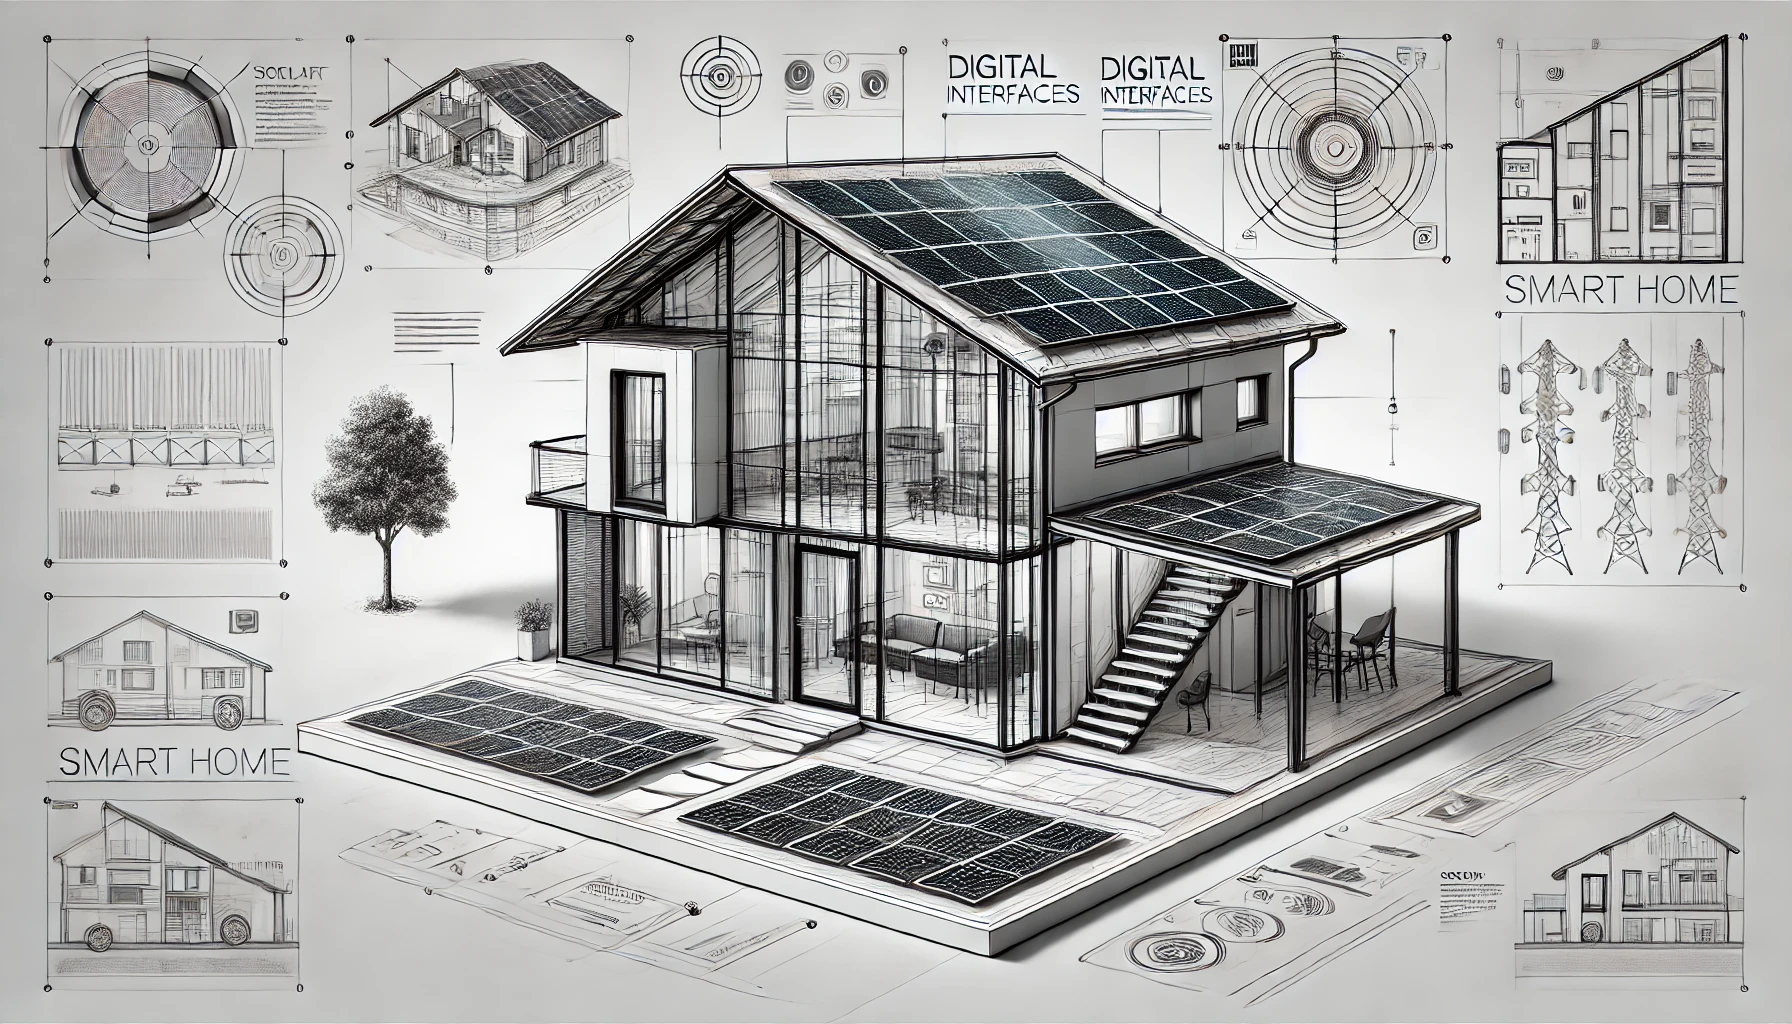
\includegraphics[width=\paperwidth]{ressources/img/logos/imageSmartHouse}} % Contenu (image de fond)
}

\usepackage[a4paper, top=2.5cm, bottom=2.5cm, left=3cm, right=2cm]{geometry}

% Pour la lisibilité, on peut utiliser le package setspace pour ajuster l'espacement entre les lignes
\usepackage{setspace}
\usetikzlibrary{positioning, decorations.pathreplacing}

\definecolor{darkWhite}{rgb}{0.94,0.94,0.94}

\lstset{
	aboveskip=3mm,
	belowskip=-2mm,
	backgroundcolor=\color{darkWhite},
	basicstyle=\footnotesize,
	breakatwhitespace=false,
	breaklines=true,
	captionpos=b,
	commentstyle=\color{red},
	deletekeywords={...},
	escapeinside={\%*}{*)},
	extendedchars=true,
	framexleftmargin=16pt,
	framextopmargin=3pt,
	framexbottommargin=6pt,
	frame=tb,
	keepspaces=true,
	keywordstyle=\color{blue},
	language=Python,
	literate=
	{²}{{\textsuperscript{2}}}1
	{⁴}{{\textsuperscript{4}}}1
	{⁶}{{\textsuperscript{6}}}1
	{⁸}{{\textsuperscript{8}}}1
	{€}{{\euro{}}}1
	{é}{{\'e}}1
	{è}{{\`{e}}}1
	{ê}{{\^{e}}}1
	{ë}{{\¨{e}}}1
	{É}{{\'{E}}}1
	{Ê}{{\^{E}}}1
	{û}{{\^{u}}}1
	{ù}{{\`{u}}}1
	{â}{{\^{a}}}1
	{à}{{\`{a}}}1
	{á}{{\'{a}}}1
	{ã}{{\~{a}}}1
	{Á}{{\'{A}}}1
	{Â}{{\^{A}}}1
	{Ã}{{\~{A}}}1
	{ç}{{\c{c}}}1
	{Ç}{{\c{C}}}1
	{õ}{{\~{o}}}1
	{ó}{{\'{o}}}1
	{ô}{{\^{o}}}1
	{Õ}{{\~{O}}}1
	{Ó}{{\'{O}}}1
	{Ô}{{\^{O}}}1
	{î}{{\^{i}}}1
	{Î}{{\^{I}}}1
	{í}{{\'{i}}}1
	{Í}{{\~{Í}}}1,
	morekeywords={*,...},
	numbers=left,
	numbersep=10pt,
	numberstyle=\tiny\color{black},
	rulecolor=\color{black},
	showspaces=false,
	showstringspaces=false,
	showtabs=false,
	stepnumber=1,
	stringstyle=\color{gray},
	tabsize=4,
	title=\lstname,
}

% Additional language definitions
\lstdefinelanguage{JavaScript}{
	keywords={typeof, new, true, false, catch, function, return, null, catch, switch, var, if, in, while, do, else, case, break},
	keywordstyle=\color{blue}\bfseries,
	ndkeywords={class, export, boolean, throw, implements, import, this},
	ndkeywordstyle=\color{darkgray}\bfseries,
	identifierstyle=\color{black},
	sensitive=false,
	comment=[l]{//},
	morecomment=[s]{/*}{*/},
	commentstyle=\color{purple}\ttfamily,
	stringstyle=\color{orange}\ttfamily,
	morestring=[b]',
	morestring=[b]"
}

\lstdefinelanguage{C}{
	keywords={auto, break, case, const, continue, default, do, double, else, enum, extern, float, for, goto, if, inline, int, long, register, restrict, return, short, signed, sizeof, static, struct, switch, typedef, union, unsigned, void, volatile, while, _Bool, _Complex, _Imaginary},
	keywordstyle=\color{blue}\bfseries,
	identifierstyle=\color{black},
	sensitive=true,
	comment=[l]{//},
	morecomment=[s]{/*}{*/},
	commentstyle=\color{green}\ttfamily,
	stringstyle=\color{red}\ttfamily,
	morestring=[b]',
	morestring=[b]"
}

\makeglossaries
\newglossaryentry{API}
{
	name=API,
	description={(Interface de Programmation d'Application) est un ensemble de protocole permettant à différentes applications logicielle d'echanger des données entre elles}
}

\newcommand{\HRule}{\rule{\linewidth}{0.5mm}}
\newcommand{\blap}[1]{\vbox to 0pt{#1\vss}}
\newcommand\AtUpperLeftCorner[3]{%
	\put(\LenToUnit{#1},\LenToUnit{\dimexpr\paperheight-#2}){\blap{#3}}%
}
\newcommand\AtUpperRightCorner[3]{%
	\put(\LenToUnit{\dimexpr\paperwidth-#1},\LenToUnit{\dimexpr\paperheight-#2}){\blap{\llap{#3}}}%
}

\title{\LARGE{Smarthouse}}
\author{\textsc{Khedhaouria} Eliès \& \textsc{Marcelet} Paul}
\date{\today}
\makeatletter



\begin{document}
	\onehalfspacing % Définit l'espacement entre les lignes à 1.5
	
	
	\begin{titlepage}
		
		
		\enlargethispage{2cm}
		
		\AddToShipoutPicture{
			\AtUpperLeftCorner{1.5cm}{1cm}{
\includegraphics[width=6.5cm]{ressources/img/logos/isimaInp.png}}
		}
		
		\begin{center}
			\vspace*{10cm}
			
			\LARGE{\textbf{Rapport d'élève Ingénieur}}\\
			\LARGE{\textbf{Stage de deuxième année}}\\
			\large{Filière:\textbf{ Sécurité} et \textbf{réseaux}} 
			\HRule
			\vspace*{0.5cm}
			\Huge{\textsc{\textbf{\@title}}}\\
			
		\end{center}
		\vspace*{2.5cm}
		Présenté par: \textbf{\@author }
		
		\vspace*{4.5cm}
		Responsable Isima: Monsieur \textbf{Alexandre GUITTON} \hspace*{2cm} Date de soutenance: \textbf{02/07/2024}\\\\
		\textbf{Campus des Cézeaux .  1 rue de la Chébarde .  TSA 60125 .  63178  Aubière CEDEX}
		
		
		
	\end{titlepage}
	\backgroundsetup{contents={}}
	\ClearShipoutPicture
	\newpage
	\tableofcontents
	\listoffigures
	
	
	\chapter{Introduction}
	\chapter{Contexte du Projet}
	\section{Expression du besoin et objectif visé}
	\section{Organisation de la conception à la création}
	
	\chapter{Analyse, Conception et Implémentation}
	\section{Infrastructure}
	\subsection{Simulation du serveur}
		\subsubsection{Mise en place d'un Broker MQTT sécurisée}
		\subsubsection{Mise en place d'une base de donnée à série temporelle}
		\subsubsection{Mise en place d'un format de donnée permettant une compatibilité entre Mosquitto et InfluxDb}
	\subsection{Simulation de la maison connecté}
		\subsection{Architecture de la simulation}
		\subsection{Implémentation du protocole MQTTs}
		\subsection{Formalisation des données envoyées}
	\section{Mise en place d'une API web}
		\subsection{Architecture de l'API}
		\subsection{Automatisation de l'authentification de chaque maison}
			\subsubsection{Mise en place d'une Base de donnée mySQL}
			\subsection{Signature automatique des certificats}
		\subsection{Filtrage et récupération des données}
			\subsubsection{Communication avec InfluxDB API}
	\section{Surveillance des données avec une interface graphique}
		\subsection{Architecture de SmartHouse Monitoring}
		\subsection{Communication avec l'API}
			\subsubsection{Authentification des maisons}
			\subsubsection{Affichage des données récupérées}
	\section{Conclusion}
		\subsection{Conclusion du projet}
		\subsection{Limites et améliorations possibles}
	


	
	
	\nocite{*}
	\bibliographystyle{unsrt}
	\bibliography{references}
	
	\clearpage
	
	\printglossaries
	
	
\end{document}